% \documentclass[11pt,a4paper]{article}
\documentclass[11pt,a4paper]{article}
%%%%%%%%%%%%%%%%%%%%%%%%% Credit %%%%%%%%%%%%%%%%%%%%%%%%

% template ini dibuat oleh martin.manullang@if.itera.ac.id untuk dipergunakan oleh seluruh sivitas akademik itera.

%%%%%%%%%%%%%%%%%%%%%%%%% PACKAGE starts HERE %%%%%%%%%%%%%%%%%%%%%%%%
\usepackage{graphicx}
\usepackage{caption}
\captionsetup[table]{name=Tabel}
\captionsetup[figure]{name=Gambar}
\usepackage{tabulary}   
% \usepackage{amsmath}
\usepackage{fancyhdr}
% \usepackage{amssymb}
% \usepackage{amsthm}
\usepackage{placeins}
% \usepackage{amsfonts}
\usepackage{graphicx}
\usepackage[all]{xy}
\usepackage{tikz}
\usepackage{verbatim}
\usepackage[left=2cm,right=2cm,top=3cm,bottom=2.5cm]{geometry}
\usepackage{hyperref}
\hypersetup{
    colorlinks,
    linkcolor={red!50!black},
    citecolor={blue!50!black},
    urlcolor={blue!80!black}
}
\usepackage{libertine}
\usepackage{libertinust1math}
\usepackage[T1]{fontenc}
\usepackage{inconsolata}

\usepackage{caption}
\usepackage{subcaption}
\usepackage{multirow}
\usepackage{psfrag}
\usepackage[T1]{fontenc}
\usepackage[scaled]{beramono}
% Enable inserting code into the document
\usepackage{listings}
\usepackage{xcolor} 
% custom color & style for listing
\definecolor{codegreen}{rgb}{0,0.6,0}
\definecolor{codegray}{rgb}{0.5,0.5,0.5}
\definecolor{codepurple}{rgb}{0.58,0,0.82}
\definecolor{backcolour}{rgb}{0.95,0.95,0.92}
\lstdefinestyle{mystyle}{
	backgroundcolor=\color{backcolour},   
	commentstyle=\color{green},
	keywordstyle=\color{codegreen},
	numberstyle=\tiny\color{codegray},
	stringstyle=\color{codepurple},
	basicstyle=\ttfamily\footnotesize,
	breakatwhitespace=false,         
	breaklines=true,                 
	captionpos=b,                    
	keepspaces=true,                 
	numbers=left,                    
	numbersep=5pt,                  
	showspaces=false,                
	showstringspaces=false,
	showtabs=false,                  
	tabsize=2
}
\lstset{style=mystyle}
\renewcommand{\lstlistingname}{Kode}
%%%%%%%%%%%%%%%%%%%%%%%%% PACKAGE ends HERE %%%%%%%%%%%%%%%%%%%%%%%%


%%%%%%%%%%%%%%%%%%%%%%%%% Data Diri %%%%%%%%%%%%%%%%%%%%%%%%
\newcommand{\stuid}{120140131}
\newcommand{\student}{\textbf{Hans Bonatua Batubara (\stuid{})}}
\newcommand{\course}{\textbf{Sistem Operasi (IF2223)}}
\newcommand{\assignment}{\textbf{02}} % tugas ke...

%%%%%%%%%%%%%%%%%%% using theorem style %%%%%%%%%%%%%%%%%%%%
\newtheorem{thm}{Theorem}
\newtheorem{lem}[thm]{Lemma}
\newtheorem{defn}[thm]{Definition}
\newtheorem{exa}[thm]{Example}
\newtheorem{rem}[thm]{Remark}
\newtheorem{coro}[thm]{Corollary}
\newtheorem{quest}{Question}[section]
%%%%%%%%%%%%%%%%%%%%%%%%%%%%%%%%%%%%%%%%
\usepackage{lipsum}%% a garbage package you don't need except to create examples.
\usepackage{fancyhdr}
\usepackage[ddmmyyyy]{datetime}
\pagestyle{fancy}
\lhead{ \student }
\rhead{ \thepage}
\cfoot{\textbf{HandsOn 2 : Synchronisation and Deadlock}} % ini untuk judul tugas
\renewcommand{\headrulewidth}{0.4pt}
\renewcommand{\footrulewidth}{0.4pt}

%%%%%%%%%%%%%%  Shortcut for usual set of numbers  %%%%%%%%%%%

\newcommand{\N}{\mathbb{N}}
\newcommand{\Z}{\mathbb{Z}}
\newcommand{\Q}{\mathbb{Q}}
\newcommand{\R}{\mathbb{R}}
\newcommand{\C}{\mathbb{C}}
\setlength\headheight{14pt}

%%%%%%%%%%%%%%%%%%%%%%%%%%%%%%%%%%%%%%%%%%%%%%%%%%%%%%%555

\begin{document}
\thispagestyle{empty}
\begin{center}
	
\includegraphics[scale = 0.15]{Figure/ifitera-header.png}
	\vspace{0.1cm}
\end{center}
\noindent
% change font family for header section only
%{\fontfamily{LinuxLibertineT-OsF}\large\selectfont 
{\large
\rule{17cm}{0.2cm}\\[0.3cm]
Nama: \student \hfill Tugas Ke: \assignment\\[0.1cm]
Mata Kuliah: \course \hfill Tanggal: \today\\
\rule{17cm}{0.05cm}
\vspace{0.1cm}
}


%%%%%%%%%%%%%%%%%%%%%%%%%%%%%%%%%%%%%%%%%%%%% BODY DOCUMENT %%%%%%%%%%%%%%%%%%%%%%%%%%%%%%%%%%%%%%%%%%%%%

\section{Tujuan HandsOn}
Tujuan dari adanya Hands On yakni adalah : 
\begin{itemize}
	\item memeahami sistem sinkronisasi dan permasalahan yang terjadi dalam sistem Operasi
	\item Memahami solusi dalam menangani \textit{critical section}
\end{itemize}
Adapun yang akan dicoba dalam Hands On adalah proses yng terkait dalam dari program dibawah ini :
		\begin{itemize}
			\item \textit{join} mengunakan \textit{semaphores}
			\item \textit{Binary semaphores}
			\item \textit{Producer Consumer}
			\item \textit{Reader / Writer}
			\item \textit{Dining Philosophers}
		\end{itemize}
\section{Ketentuan Praktikum}
Pada praktikum atau Hands On pada minggu ini akan pengerjaan hands on dilakukan dengan beberapa tahap yaitu :
\begin{itemize}
    \item Tahap pertama adalah proses menginstall dan cloning code yang apa pada github
        \begin{lstlisting}[language=Bash,label={labelkode}]
        sudo apt install git
        git clone https://github.com/remzi-arpacidusseau/ostep-code.git
        \end{lstlisting}
        pada tahap ini langkah pertama adalah menginstall git dan selanjutnya dipakai untuk melakukan clone, tujuan dari tahap ini untuk mengambil code yang ingin diuji coba pada praktikum kali ini
    \item Tahap kedua adalah proses untuk mengakses file yang ingin dicoba pada praktikum dalam mengakses cd atau change directory untuk mengakses file hasil clone yang ada ditelah ada dalam perangkat kita.
    \begin{lstlisting}[language=Bash,label={labelkode}]
        cd ostep-code
        ls
        cd threads-sema
        make
        ls
        ./<file>
        \end{lstlisting}
        pada tahap ini file akan dibuat dengan sintax make adpun file yang dibuat berada pada file threads-sema, sehingga isi dari file itu dapat diakses
    
\end{itemize}
\section{\textit{Fork/Join}}
\subsection{souce code}
\begin{lstlisting}[language=C]
	sem_t s;

	void *child(void *arg) {
		sleep(2);
		printf("child\n");
		Sem_post(&s); // signal here: child is done
		return NULL;
	}

	int main(int argc, char *argv[]) {
		Sem_init(&s, 0); 
		printf("parent: begin\n");
		pthread_t c;
		Pthread_create(&c, NULL, child, NULL);
		Sem_wait(&s); // wait here for child
		printf("parent: end\n");
		return 0;
	}
    

\end{lstlisting}

\vspace{2cm}
\subsection*{output}
\begin{figure}[h]
	\centering
	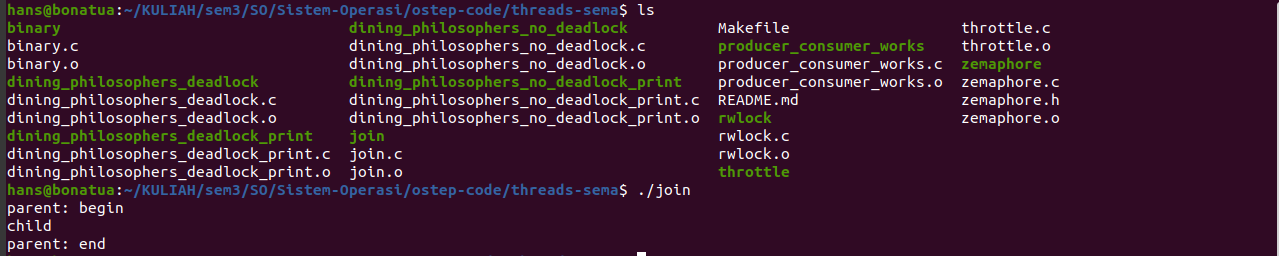
\includegraphics[width=0.8\textwidth]{Figure/testing/percobaan-join.png}
	\caption{Fork/Join}
\end{figure}

\subsection{penjelasan}
Semaphore pada dasar adalah sebuah bentuk dari data komputer yang berfungsi untuk menyelaraskan atau melakukan sinkronisasi yang bertujuan memerintahkan suatu program untuk menjalan suatu proses. salah satu bentuk implementasi dari semaphore adalah saat ada suatu  \textit{thread} yang menunggu suatu \textit{list}, supaya \textit{list} tidak kosong atau bernilai \textit{null} dalam proses  kerjanya. Pada kondisi yang demikian semaphore tadi bekerja dengakn mekanisme semaphore akan memberi nilai inisiasi menjadi 0 oleh \textit{Sem init}, pada moment ini juga semaphore akan dibagi antara \textit{threads} pada kondisi yang sama, setelah pembuatan \textit{threads} selesai akan dilanjukan dengan proses alan dilanjutkan dengan memanggil fungsi \textit{child} semaphore akan memberikan sinyal bahwa proses \textit{child} sudah selesai dan akan melakukan pengembalian nilai \textit{return}. Setelah menyelesaikan proses pada fungsi \textit{child} semaphore akan mengakhiri program dengan mengeluarkan \textit{output} yakni "parent:end" 

Pada penerapan terdapat fungsi \textit{Sem wait} dan \textit{Sem post} yang berfungsi untuk menunggu perubahan kondisi dari \textit{parent} menjadi \textit{child} selesai dieksekusi. Pada salah satu bagian kode tersebut terlihat \textit{value} semaphore harus berubah terlebih dahulu 0 hal ini tidak dilakukan akan membuat parent memanggil fungsi \textit{Sem wait} terlebih dahulu sebelum child selesai memanggil fungsi \textit{Sem post}. Dan dari kondisi tersenut, dapat diketahui bila \textit{value} semaphore dapat lebih dari 0 akan melakukan pengurangan untuk melakukan \textit{sleeps} selama 2 detik. Apabila \textit{value} semaphore sama dengan 0, maka program mulai menjalankan parent dan selesai


\section{\textit{Binary Semaphores}}
\subsection*{souce code}
\begin{lstlisting}[language = C]

	volatile int counter = 0;

	void *child(void *arg) {
		int i;
		for (i = 0; i < 10000000; i++) {
		Sem_wait(&mutex);
		counter++;
		Sem_post(&mutex);
		}
		return NULL;
	}

	int main(int argc, char *argv[]) {
		Sem_init(&mutex, 1); 
		pthread_t c1, c2;
		Pthread_create(&c1, NULL, child, NULL);
		Pthread_create(&c2, NULL, child, NULL);
		Pthread_join(c1, NULL);
		Pthread_join(c2, NULL);
		printf("result: %d (should be 20000000)\n", counter);
		return 0;
	}
\end{lstlisting}
\subsection*{output}
\begin{figure}[h]
	\centering
	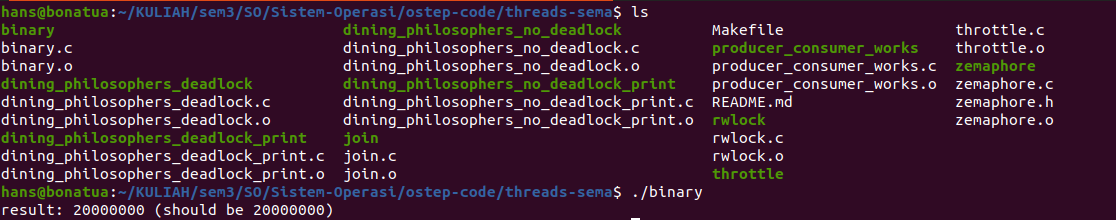
\includegraphics[width=0.8\textwidth]{Figure/testing/percobaan-binary.png}
	\caption{Binary Semaphores}
\end{figure}

\subsection{penjelasan}
dari kode diatas terdapat variable \textit{Sem t mutex} atau dapat disebut \textit{mutual exclusion} yang berfungsi mengatur pemakaian \textit{resourse}. variable \textit{mutex} bertujuan agr mencegah terjadinya \textit{race condition}. Pada dasarnya  kita mendefinisikan dan menginisialisasikan semaphore \textit{mutex} tesebut dengan value sebesar 1,selanjutnya dibuatlah \textit{thread} yang berinisial c1 dan c2 yang mana akan dipakai dalam menjalankan fungsi \textit{child}. dan dilanjutkan dengan menginisiaisi i pada perulangan sampai nilai i kurang dari 10000000 yang dimana akan menjalankan \textit{Sem wait} dan di saat proses itu juga \textit{value} akan berkurang dan akan memulai terjadi kondisi \textit{critical section}, yang akan berakibat penambahan nilai \textit{counter} yang kemudian semaphore memproses \textit{calling} dengan menambah value dari semaphore. Proses tersebut menjadi sebuah tanda \textit{critical section} sudah selesai. Berikutnya, program akan proses \textit{looping} tersebut hingga syarat kondisi tercapai yang  dilanjutkan oleh thread c2 yang melakukan fungsi \textit{child}. Jika semua proses sudah terpenuhi, maka akan memulai return ke fungsi \textit{main} yang akan menampilkan hasil dari \textit{counter} yang telah dijalankan dengan menampilkan nilai keluaran yang bernilai 20000000

\section{\textit{Producer Consumer}}
\subsection{souce code}
\begin{lstlisting}[language = C]
	int max;
	int loops;
	int *buffer;

	int use  = 0;
	int fill = 0;

	sem_t empty;
	sem_t full;
	sem_t mutex;

	#define CMAX (10)
	int consumers = 1;

	void do_fill(int value) {
		buffer[fill] = value;
		fill++;
		if (fill == max)
		fill = 0;
	}

	int do_get() {
		int tmp = buffer[use];
		use++;
		if (use == max)
		use = 0;
		return tmp;
	}

	void *producer(void *arg) {
		int i;
		for (i = 0; i < loops; i++) {
		Sem_wait(&empty);
		Sem_wait(&mutex);
		do_fill(i);
		Sem_post(&mutex);
		Sem_post(&full);
		}

		// end case
		for (i = 0; i < consumers; i++) {
		Sem_wait(&empty);
		Sem_wait(&mutex);
		do_fill(-1);
		Sem_post(&mutex);
		Sem_post(&full);
		}

		return NULL;
	}
																				
	void *consumer(void *arg) {
		int tmp = 0;
		while (tmp != -1) {
		Sem_wait(&full);
		Sem_wait(&mutex);
		tmp = do_get();
		Sem_post(&mutex);
		Sem_post(&empty);
		printf("%lld %d\n", (long long int) arg, tmp);
		}
		return NULL;
	}

	int main(int argc, char *argv[]) {
		if (argc != 4) {
		fprintf(stderr, "usage: %s <buffersize> <loops> <consumers>\n", argv[0]);
		exit(1);
		}
		max   = atoi(argv[1]);
		loops = atoi(argv[2]);
		consumers = atoi(argv[3]);
		assert(consumers <= CMAX);

		buffer = (int *) malloc(max * sizeof(int));
		assert(buffer != NULL);
		int i;
		for (i = 0; i < max; i++) {
		buffer[i] = 0;
		}

		Sem_init(&empty, max); // max are empty 
		Sem_init(&full, 0);    // 0 are full
		Sem_init(&mutex, 1);   // mutex

		pthread_t pid, cid[CMAX];
		Pthread_create(&pid, NULL, producer, NULL); 
		for (i = 0; i < consumers; i++) {
		Pthread_create(&cid[i], NULL, consumer, (void *) (long long int) i); 
		}
		Pthread_join(pid, NULL); 
		for (i = 0; i < consumers; i++) {
		Pthread_join(cid[i], NULL); 
		}
		return 0;
	}
\end{lstlisting}

\subsection*{output}
\begin{figure}[h]
	\centering
	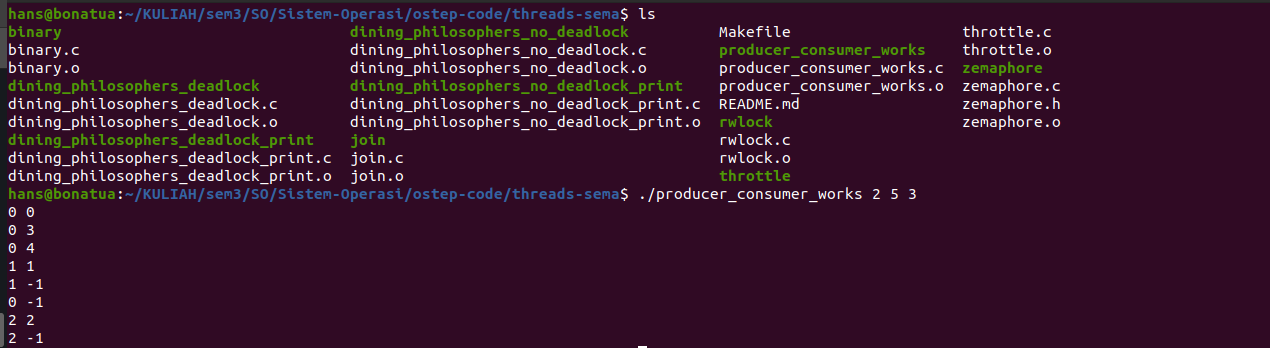
\includegraphics[width=0.8\textwidth]{Figure/testing/PercobaanProducer.png}
	\caption{Producer Consumer}
\end{figure}
\vspace{1cm}
\subsection{penjelasan}
Pada implementasi pada program \textit{Producer/consumer} dapat disebut dengan \textit{bounded buffer}. Isi program memanggil, menghambat konsumer, dan menunggu \textit{thread} yang lain supaya dapat memanggil \textit{Sem post} saat kondisi \textit{full}. Kemudian, program dapat menjalankan fungsi \textit{Procedur} yang berfungsi memanggil \textit{Sem wait(empty)} dan \textit{Sem post(mutex)}.Dan pada fungsi \textit{Procedur} juga terus berjalan sampai tercapai kondisi \textit{empty} yang menjadi \textit{max}. \textit{Procedur} akan melakukab pengisian dengan memakai fungsi \textit{do fill} di \textit{entry} pertama pada \textit{buffer} selanjutnya setelah \textit{empty} akan terus berkurang hinggaa nilai = 0. kemudian, \textit{procedur} akan terus berjalan sampai sutu saat nanti akan memanggil \textit{Sem post(mutex)} dan\textit{Sem post(full)} yang dimana akan mengubah nilai \textit{value empty} dari nilai -1 menjadi 0. Sehingga, Consumer akan melakukan fungsi perulangan (\textit{looping}) dan menutup dengan \textit{value empty} semaphore bernilai kosong  
    Jika kondisi \textit{procedur interrupted}, maka fungsi \textit{Consumer}
mulai berjalan dengan mengembalikan nilai dari \textit{Sem wait(full)}, lalu akan menggunakan \textit{buffer} oleh berjalannya fungsi \textit{do get}. kedua kondisi \textit{producer} akan mengalami \textit{interrupted} apabila keduanya menjalankan fungsi \textit{do fill} pada waktu yang sama. kondisi \textit{interruped} juga terjai jika \textit{procedur}  yang pertama mengisi \textit{entry buffer} pertama kali, saat belum selesai dalam kesempatan mengisinya, maka \textit{procedur} pertama akan ter-\textit{interruped}. Pada kondisi yang demikian \textit{procedur} yang lain akan mengantikan oleh \textit{procedur} kedua dimana akan menjalan kembali fungsi \textit{do fill}
yang akan memasukkan elemen \textit{buffer}, kondisi tersebut berarti bahwa data yang sebelumnya akan terganti dengan yang baru. Oleh karena itu dibutuhkan \textit{binary semaphore} dan ditambahkan \textit{locks} agar menghindari \textit{deadlock}. Dari kondisi demikian \textit{consumer} menjalankan yang pertama dengan memanggil \textit{Sem wait (full)} akibat dari kosongnya data. Dampak yang diakibatkan dengan pemanggilan tersebut, \textit{consumer threads} akan tertaham mem-\textit{block}, agar \textit{procedur} berjalan yang akan menjalankan \textit{consumer thread}  dan memanggil \textit{Sem wait(mutex)} dengan producer yang mengalamistuck. Pada program di atas terdapat sebuah cycle yang mudah, \textit{consumer} menahan \textit{mutex} agar menunggu untuk diberikan sinyal full. Faktanya  \textit{producer} dapat memanggil sinyal full, akan tetapi tetap menunggu hingga \textit{consumer} dan \textit{producer} mengalami \textit{deadlock}. Oleh sebab itu, diperlukan pengurangan \textit{lock} dengan memindahkan mutex dan melepaskannya pada sekitar \textit{critical section} akan menghasilkan \textit{working bounded buffer} .

\section{\textit{Reader / Writer}}
\subsection{souce code}
\begin{lstlisting}[language = C]		
	int read_loops;
	int write_loops;
	int counter = 0;

	rwlock_t mutex;

	void *reader(void *arg) {
		int i;
		int local = 0;
		for (i = 0; i < read_loops; i++) {
		rwlock_acquire_readlock(&mutex);
		local = counter;
		rwlock_release_readlock(&mutex);
		printf("read %d\n", local);
		}
		printf("read done: %d\n", local);
		return NULL;
	}

	void *writer(void *arg) {
		int i;
		for (i = 0; i < write_loops; i++) {
		rwlock_acquire_writelock(&mutex);
		counter++;
		rwlock_release_writelock(&mutex);
		}
		printf("write done\n");
		return NULL;
	}

	int main(int argc, char *argv[]) {
		if (argc != 3) {
		fprintf(stderr, "usage: rwlock readloops writeloops\n");
		exit(1);
		}
		read_loops = atoi(argv[1]);
		write_loops = atoi(argv[2]);
		
		rwlock_init(&mutex); 
		pthread_t c1, c2;
		Pthread_create(&c1, NULL, reader, NULL);
		Pthread_create(&c2, NULL, writer, NULL);
		Pthread_join(c1, NULL);
		Pthread_join(c2, NULL);
		printf("all done\n");
		return 0;
	}
\end{lstlisting}

\subsection*{output}
\begin{figure}[h]
\centering
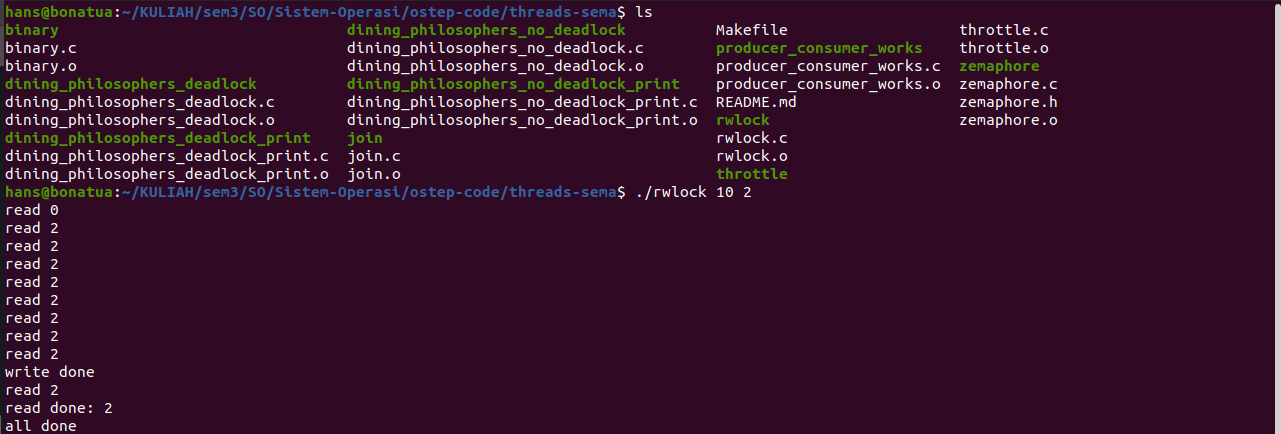
\includegraphics[width=0.8\textwidth]{Figure/testing/PercobaanRwlock.png}
\caption{Reader / Writer}
\end{figure}
\subsection{penjelasan}
Pada penerapan program \textit{Reader/ writer locks}, dapat dilihat bahwa terdapat suatu \textit{classic problem} dari \textit{flexible locking primitive} yang memperlihatkan bahwa untuk mengakses struktur data yang berbeda diperlukan kunci yang besifat unik, yang berfungsi sebagai tipe operasi seperti halnya \textit{reader/writer locks}. Apabila suatu kondisi \textit{thread} mengalami pembaruan struktur datanya, agar tetap terpasang dan sinkron dibutuhkan operasi sinkronisasi yakni\textit{rwlock acquire writelock} yang man berfungsi dalam mendapatkan \textit{writelock} dan \textit{rwlock release writelock} untuk melepaskannya. Secara umumnya , semaphore \textit{writelock} yang memastikan hanya satu \textit{writer} yang mendapatkan \textit{lock} dan memperbarui struktur data dengan mengakses \textit{critical section}
      Ketika \textit{lock} didaptkan pada suatu kondisi, \textit{reader} akan
menjadi pertama yang akan mendapatkan \textit{lock} dan mulai menambahkan variabel pembaca agar dapat melacak pembaca yang ada pada struktur data. hal utama yang tidak boleh tidak diperhatikan bahwa \textit{rwlock acquire readlock} dapat bekerja saat pembaca pertama mendapatkan \textit{lock} dan \textit{writelock} dengan memanggil \textit{Sem wait} ketika semaphore \textit{writelock} yang akan dilepaskan \textit{lock}-nya saat memanggil kembali \textit{Sem post} . Kemudian, saat semua threads dibuthkan mendapatkan \textit{writelock} harus menunggu hingga semua reader telah selesai bekerja. Saat urutan terakhir keluar dari kondisi \textit{critical section}, akan kembali memanggil \textit{Sem post} yang ada pada \textit{writelock} dan mulai kembali mengaktifkannya \textit{writer}  dengan menunggu dapatnya \textit{lock}. Hingga pada akhirnya, pencatatan \textit{readwriter locks} wajib dilakukan secara seksama karena hal tersebut mengakibatkan adaanya penambahan \textit{overhead} dan tidak menambah performa yang berguna sebagai komparansi di \textit{simple} dan \textit{fast locking primptive}


\section{\textit{Dining Philosophers}}
\subsection{\textit{Dining Philosophers Deadlock}}
\subsubsection[shotr]{source code}
\begin{lstlisting}[language = C]

	void space(int s) {
		Sem_wait(&print_lock);
		int i;
		for (i = 0; i < s * 10; i++)
		printf(" ");
	}
	
	void space_end() {
		Sem_post(&print_lock);
	}
	
	int left(int p)  {
		return p;
	}
	
	int right(int p) {
		return (p + 1) % 5;
	}
	
	void get_forks(int p) {
		space(p); printf("%d: try %d\n", p, left(p)); space_end();
		Sem_wait(&forks[left(p)]);
		space(p); printf("%d: try %d\n", p, right(p)); space_end();
		Sem_wait(&forks[right(p)]);
	}
	
	void put_forks(int p) {
		Sem_post(&forks[left(p)]);
		Sem_post(&forks[right(p)]);
	}
	
	void think() {
		return;
	}
	
	void eat() {
		return;
	}
	
	void *philosopher(void *arg) {
		arg_t *args = (arg_t *) arg;
	
		space(args->thread_id); printf("%d: start\n", args->thread_id); space_end();
	
		int i;
		for (i = 0; i < args->num_loops; i++) {
		space(args->thread_id); printf("%d: think\n", args->thread_id); space_end();
		think();
		get_forks(args->thread_id);
		space(args->thread_id); printf("%d: eat\n", args->thread_id); space_end();
		eat();
		put_forks(args->thread_id);
		space(args->thread_id); printf("%d: done\n", args->thread_id); space_end();
		}
		return NULL;
	}
																				 
	int main(int argc, char *argv[]) {
		if (argc != 2) {
		fprintf(stderr, "usage: dining_philosophers <num_loops>\n");
		exit(1);
		}
		printf("dining: started\n");
		
		int i;
		for (i = 0; i < 5; i++) 
		Sem_init(&forks[i], 1);
		Sem_init(&print_lock, 1);
	
		pthread_t p[5];
		arg_t a[5];
		for (i = 0; i < 5; i++) {
		a[i].num_loops = atoi(argv[1]);
		a[i].thread_id = i;
		Pthread_create(&p[i], NULL, philosopher, &a[i]);
		}
	
		for (i = 0; i < 5; i++) 
		Pthread_join(p[i], NULL); 
	
		printf("dining: finished\n");
		return 0;
	}
\end{lstlisting}

\subsubsection*{output}
\begin{figure}[h]
	\centering
	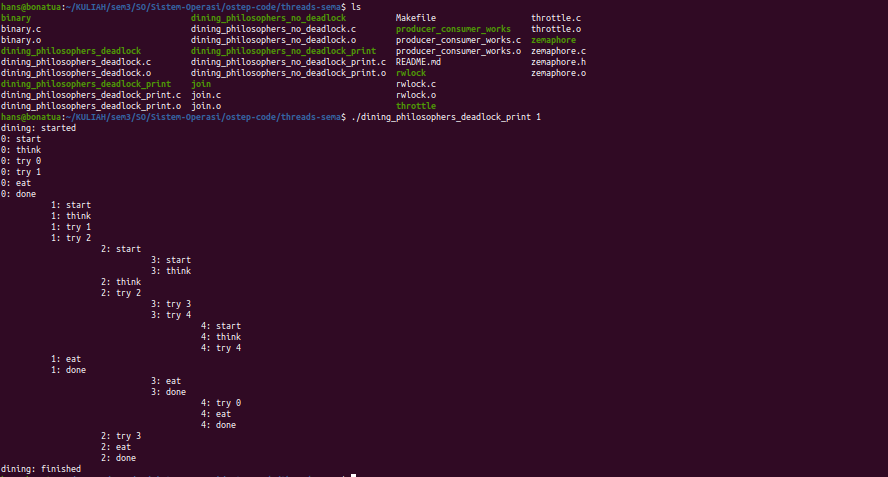
\includegraphics[width=0.8\textwidth]{Figure/testing/Percobaan-deadlock.png}
	\caption{Dining Philosophers Deadlock}
\end{figure}

\subsubsection{penjelasan}
Pada penerapan program \textit{Dining Philosopher Deadlock} mempunyai hal yang menarik terkait adanya suatu masalah yang bersifat konkurensi yang dulu terkenal karena hanya dapat diselesaikan oleh sebuah alogaritma yakni alogaritma djikstra (\textit{djikstra algorithm}. Masalah ini menjadi menarik menjadi alasan kenapa disebut program memiliki ini \textit{Philosophers problem}. yang dimana ketentuan ketika ada 5 orang \textit{philosopher} yang duduk melingkar pada sebuah meja bundar terdapat sepasang \textit{philosopher single fork} yang dimana untuk memulai suatu kegiatan dibutuhkan sepasang \textit{forks} didua tempat berbeda. Oleh karena itu diperlukan fungsi bantu yang disebut \textit{left} dan \textit{right}. Kondisi ketika salah satu \textit{philosopher} merunjuk pada suatu arah, ia akan mengajak bagian yang lain untuk mengatasi persoalan pada bagian lain 

\subsection {\textit{Dining Philosophers no Deadlock}}
\subsubsection{source code}
\begin{lstlisting}[language = C]
	void space(int s) {
		Sem_wait(&print_lock);
		int i;
		for (i = 0; i < s * 10; i++)
		printf(" ");
	}
	
	void space_end() {
		Sem_post(&print_lock);
	}
	
	int left(int p)  {
		return p;
	}
	
	int right(int p) {
		return (p + 1) % 5;
	}
	
	void get_forks(int p) {
		if (p == 4) {
		space(p); printf("4 try %d\n", right(p)); space_end();
		Sem_wait(&forks[right(p)]);
		space(p); printf("4 try %d\n", left(p)); space_end();
		Sem_wait(&forks[left(p)]);
		} else {
		space(p); printf("try %d\n", left(p)); space_end();
		Sem_wait(&forks[left(p)]);
		space(p); printf("try %d\n", right(p)); space_end();
		Sem_wait(&forks[right(p)]);
		}
	}
	
	void put_forks(int p) {
		Sem_post(&forks[left(p)]);
		Sem_post(&forks[right(p)]);
	}
	
	void think() {
		return;
	}
	
	void eat() {
		return;
	}
	
	void *philosopher(void *arg) {
		arg_t *args = (arg_t *) arg;
	
		space(args->thread_id); printf("%d: start\n", args->thread_id); space_end();
	
		int i;
		for (i = 0; i < args->num_loops; i++) {
		space(args->thread_id); printf("%d: think\n", args->thread_id); space_end();
		think();
		get_forks(args->thread_id);
		space(args->thread_id); printf("%d: eat\n", args->thread_id); space_end();
		eat();
		put_forks(args->thread_id);
		space(args->thread_id); printf("%d: done\n", args->thread_id); space_end();
		}
		return NULL;
	}
																				 
	int main(int argc, char *argv[]) {
		if (argc != 2) {
		fprintf(stderr, "usage: dining_philosophers <num_loops>\n");
		exit(1);
		}
		printf("dining: started\n");
		
		int i;
		for (i = 0; i < 5; i++) 
		Sem_init(&forks[i], 1);
		Sem_init(&print_lock, 1);
	
		pthread_t p[5];
		arg_t a[5];
		for (i = 0; i < 5; i++) {
		a[i].num_loops = atoi(argv[1]);
		a[i].thread_id = i;
		Pthread_create(&p[i], NULL, philosopher, &a[i]);
		}
	
		for (i = 0; i < 5; i++) 
		Pthread_join(p[i], NULL); 
	
		printf("dining: finished\n");
		return 0;
	}	
\end{lstlisting}
\newpage
\subsubsection*{output}
\begin{figure}[h]
	\centering
	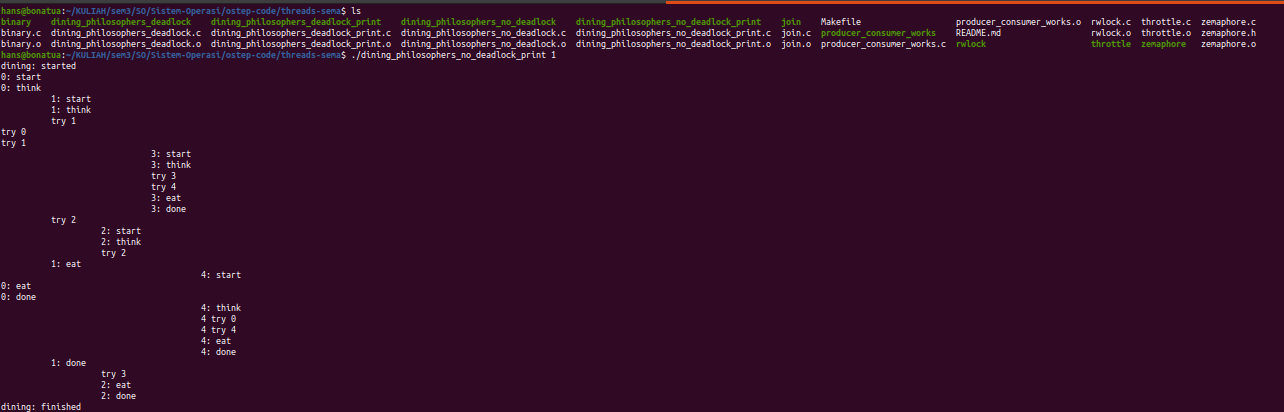
\includegraphics[width=0.8\textwidth]{Figure/testing/Percobaan-Nodeadlock.png}
	\caption{Dining Philosophers no Deadlock}
\end{figure}

\newpage
\vspace{3cm}
\subsubsection{penjelasan}
Pada penerapan program \textit{Dining Philosopher No Deadlock} yang ada di atas, menjelaskan terkait percobaan menginstall setiap \textit{fork array} agar selalu bernilai satu. Hal yang menjadi perhatiaan adalah \textit{philosopher} mempunyai angka dan juga dapat menuliskan \textit{get froks} dan \textit{put forks} secara berulang. kemudian untuk mengakses dan melepas diperlukan \textit{lock} untuk mendapati \textit{lock} yang lain dan akan terus menerus bergantian, tetapi kondisi ini terhambat karena adanya \textit{deadlock}, yang berakibat terhambatnya proses pertukaran \textit{forks} dan juga menghambat 1 \textit{fork} dan 1 \textit{fork} yang lain hal ini terjadi ketika 1 \textit{fork} diambil maka akan menaham \textit{fork} agar menunggu sampai selamanya. Dari permasalahan diatas alogaritma djikstra (\textit{djikstra algorithm} menemukan alternatif cara untuk mengatasi masalah tersebut yakni dengan cara menganti \textit{philoshoper}, dengan asumsi setiap \textit{philoshoper} yang lain melalui aturan yang berbeda dengan \textit{philoshoper} yang sebelumnya sehingga tidak ada \textit{philoshope}yang menunggu. 
\newpage

\section{kesimpulan}
Pada Hands on 2, saya mendapatkan suatu kesimpulan bahwasanya setiap suatu perintah tidak dapat berdiri sendiri, ketika suatu program lain bekerja  maka dalam membuat program tersebut bekerja diperlukan program pendukung yang saling tersinkronisasi dengan yang lain yang mendorong program utama agar mendapat hasil yang maksimal. Setiap poin didalam percobaan ini memiliki dasar yang sama yakni \textit{Synchronisation and Deadlock} yang harus saling terintegrasi agar tidak terjadi stuck pada program
\section{link laporan dan berkas}
\begin{itemize}
	\item Link github :\href{}{}
\end{itemize}




\end{document}
